\documentclass[]{article}
\usepackage{amsmath,amssymb}
\usepackage{graphicx}

\usepackage[utf8]{inputenc}
\usepackage[T1]{fontenc}
\usepackage[russian]{babel}

%opening
\title{О непереполненном базисе скалярных и смешанных произведений сигма-матриц}
\author{Олег Лычковский, Филипп Усков}

\begin{document}

\maketitle

\begin{abstract}
Исследуется вопрос полном вращательно-инвариантном операторном базисе для спиновых систем.  Вопрос важен для оценки энергии основного состояния в купратах.

\end{abstract}

\section{Введение}

Есть купраты (антиферромагнетики). У них гамильтониан вот такой:
$$H=-J\sum_{<i,j>}\vec\sigma_i\vec\sigma_j$$
где $<i,j>$ означает соседние спины в решетке, как на рис. 1,2
\begin{figure}[h]
	\begin{minipage}{6pc}
		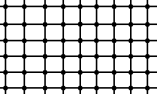
\includegraphics[width=6pc]{sqlattice.png}
	\end{minipage}\hspace{2pc}%
	\begin{minipage}{5pc}
		\caption{\label{label} 2d квадратная решетка.}
	\end{minipage}\hspace{2pc}%
	\begin{minipage}{6pc}
		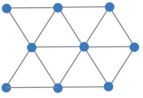
\includegraphics[width=6pc]{triangle-lattice.png}
	\end{minipage}\hspace{2pc}%
	\begin{minipage}{5pc}
		\caption{\label{label} 2d треугольная решетка.}
	\end{minipage} 
\end{figure}

И важно находить энергию основоного состояния (на один спин).
Оценить эту энергию сверху можно по формуле $E_{\rm gs} \leqslant \langle \Psi|H| \Psi \rangle$.
Оценить снизу можно разбивая кристалл на кластеры\cite{Anderson}, а также вариационно \cite{variational} 
$${E_{gs\;full}}/N\;=\frac{d}{m}{E_{gs\;cl}}$$
где
\begin{itemize}
	\item $N$ - количество спинов в решетке
	\item $M$ - количество кластров
	\item $d$ - количество связей на 1 спин
	\item $m$ - количество связей в кластере
\end{itemize}
$$M = \frac{{Nd}}{m} \label{MNdm} $$

Энергию основного состояния кластера можно находить из уравнения Шредингера 
$$H \rho = E \rho$$
На $\rho$ как на матрицу плотности накладываются ограничения: самосопряженность, единичный след, неотрицательность.
$${\rho ^ + } = \rho ;\qquad \mathop{\rm{tr}}\rho  = 1;\qquad  \rho  \geqslant 0$$
Этого можно добиться введя параметр тау: 
$$\rho  = \frac{{{\tau ^2}}}{{\mathop{\rm{tr}}{\tau ^2}}};\qquad {\tau ^ + } = \tau $$
где на $\tau$ накладывается только самосопряженность.

Далее мы вводим базис для $\tau$, и раскладываем ее по нему.
$$\tau=b_i A_i$$
Поскольку система сферически симметрична, то в качестве базисных элементов можно выбрать всевозможные произведения 
скалярных и смешанных произведений сигма-матриц, а т.к. система еще симметрична по обращению времени, то можно оставить только скалярные произведения.
$$A_i=\{ 1,  \;\;({\bf \sigma}_j{\bf\sigma}_k), \;\;
({\bf \sigma}_j{\bf\sigma}_k)({\bf \sigma}_l{\bf\sigma}_m)\;\;,\;\;...\}$$
Этот базис не только не ортогонален, но и переполнен.

\section{Цель и ход работы}
Мы захотели получить этот базис в непереполненном виде, чтобы немного сократить объем вычилений.

%Мы нашли статью \cite{basis_f} про "базис f", но через год, когда мы ее всё-таки прочитали, оказалось что это вообще не имеет ни какого отношения к нашему базису.

Мы решили посчитать сколько же на самом деле линейнонезависимых векторов в нашем базисе для небольшого числа спинов,
нашли эту последовательность на OEIS, 
и нашли статью, которая описывает, как строить непереполненный базис, и вот что там говориться:

\section{Построение непереполненного базиса \cite{source_article}}
Элементы базиса будем называть табличками. Эти таблички заполняются номерами спинов.

Столбец длины 3 мы интерпретируем как смешанное произведение.
$$ \begin{tabular}{ | l | }
\hline
1 \\ \hline
2 \\ \hline
3 \\
\hline
\end{tabular} = (\vec \sigma_1, \vec \sigma_2, \vec \sigma_3) $$
Пару столбцов мы интерпретируем как определитель скалярных произведений (или, что то же самое, обобщенный символ Кронекера).
$$ \begin{tabular}{ |l|l| }
\hline
1 & 4 \\ \hline
2 & 5\\ 
\hline
\end{tabular}
 = 
\begin{vmatrix}
(\vec\sigma_1,\vec\sigma_4) & (\vec\sigma_1,\vec\sigma_5)\\
(\vec\sigma_2,\vec\sigma_4) & (\vec\sigma_2,\vec\sigma_5)\\
\end{vmatrix}
$$
в частности

пара столбцов длины 1 это просто скалярное произведение
$$\begin{tabular}{ |l|l| }
\hline
1 & 2 \\
\hline
\end{tabular}
= (\vec \sigma_1, \vec \sigma_2)
$$
пара столбцов длины 3 равна произведению двух смешанных произведений (каждое соответствует  своему столбцу)
$$ \begin{tabular}{ |l|l| }
\hline
1 & 4 \\ \hline
2 & 5\\ \hline
3 & 6\\
\hline
\end{tabular}
= 
\begin{vmatrix}
(\vec\sigma_1,\vec\sigma_4) & (\vec\sigma_1,\vec\sigma_5) & (\vec\sigma_1,\vec\sigma_6) \\
(\vec\sigma_2,\vec\sigma_4) & (\vec\sigma_2,\vec\sigma_5) & (\vec\sigma_2,\vec\sigma_6) \\
(\vec\sigma_3,\vec\sigma_4) & (\vec\sigma_3,\vec\sigma_5) & (\vec\sigma_3,\vec\sigma_6) \\
\end{vmatrix}
=
(\vec \sigma_1, \vec \sigma_2, \vec \sigma_3)
(\vec \sigma_4, \vec \sigma_5, \vec \sigma_6)
$$

В базис войдут элементы, удовлетворяющие следующим критериям:
\begin{itemize}
	\item кажда строка в табличке содержит число ячеек не больше чем в предыдущей строке
	\item строк не больше 3
	\item Для четного числа спинов:
	\begin{itemize}
		\item столбцы разбиваются на пары, длины столбцов в каждой паре совпадают
	\end{itemize}
	\item Для нечетного числа спинов:
	\begin{itemize}
		\item в начале таблички добавляется столбец длины 3
		\item оставшиеся N-3 ячейки делаем как для четного числа
	\end{itemize}
	\item после чего заполняем эти табличками различающимися номерами спинов так, чтобы каждая строка и каждый столбец был отсортирован
\end{itemize}

Была написана функция \cite{basis_gen_code}, которая генерирует все возможные элементы базиса, и их число совпало с формулой из статьи
$$Q_n = \sum_{r=0}^{[n/2]}\frac{n!(3r-n+1)}{(n-2r)!r!(r+1)!}.$$
Ранее нами была обнаружена гипотеза, что пара столбцов длины 4 =0, и что этим объясняются все линейные зависимости в базисе с четным числом спинов.
$$ \begin{tabular}{ |l|l| }
\hline
1 & 5 \\ \hline
2 & 6\\ \hline
3 & 7\\ \hline
4 & 8\\
\hline
\end{tabular}=0 .
$$
Был замечен факт, что если для четного числа спинов сгененрировать все возможные таблички без ограничения числа строк,
то их общее число оказалось равно количеству элементов нашего исходного переполненного базиса
$$N_n=\begin{cases}
\frac{n!}{2^{n/2}(n/2)!} & (n=2k)\\
\frac{n!}{3\dot 2^{(n-1)/2}((n-3)/2)!} & (n=2k+1)
\end{cases}$$
откуда можно сделать вывод, что скорее всего все таблички, у которых число строк больше 4 (они =0), дают все линейные зависимости в исходном базисе.
Для нечетного количества спинов аналогичный факт нами пока не придуман.

\section{Планы применения непереполненного базиса к уравнению Шредингера}
Если вернуться к иходной задаче $H \rho = E \rho$, то 
нам требуется умножать элементы нашего базиса (из $\rho$) на скалярные произведения (из $H$), и полученный результат вновь раскладывать по базису.
Для переполненного базиса это было реализовано ранее (и описано в предыдущих статьях \cite{variational}.
Для нового непереполненного базиса это сделать пока не удалось (так чтобы не при этом не переходить к старому переполненному базису, что сводит на нет преимущества нового непереполненного базиса)

\begin{thebibliography}{3}
	\bibitem{source_article}
	D. L. Andrews and T. Thirunamachandran, On three-dimensional rotational averages, 1977
	
	\bibitem{variational}
	Filipp Uskov, Oleg Lychkovskiy, A variational lower bound on the ground state of a 	many-body system and the squaring parametrization of density matrices, 2018
	
	\bibitem{Anderson} Anderson PW 1951
	Limits on the energy of the antiferromagnetic Ground State
	{\it Phys. Rev.} {\bf 83(6)} 1260
	
	\bibitem{basis_gen_code}
	https://github.com/FeelUsM/ScalarMixedSpins/blob/master/tables.nb
	
	\bibitem{variational_method}
	Filipp Uskov, Oleg Lychkovskiy, A variational lower bound on the ground state of a many-body system and the squaring parametrization of density matrices, .....
	
	\bibitem{anderson}
	Anderson PW 1951 Limits on the energy of the antiferromagnetic Ground State Phys. Rev. 83(6) 1260
	
	\bibitem{basis_f}
	P. Grabowski and Pierre Mathieu, Quantum Integrals of Motion for the Heisenberg Spin Chain, LAVAL-PHY-94-20
	
\end{thebibliography}

\end{document}
